\makeatletter
\def\input@path{{styles/}}
\makeatother
\ifx\bookMode\undefined%
    %-----------------------------------------------------------------------------
% Master Prefix File for Randomized Algorithms Class Notes & Book
% Unified self-contained configuration for LuaLaTeX and XeLaTeX with Memoir
%-----------------------------------------------------------------------------

\RequirePackage{iftex}
\ifPDFTeX
  \PackageError{engine-guard}{This document requires LuaLaTeX or XeLaTeX}{%
    Please recompile using LuaLaTeX or XeLaTeX instead of pdfLaTeX.%
  }
  \stop
\fi

% Always use memoir
\documentclass[12pt,oneside,fleqn]{memoir}

%-----------------------------------------------------------------------------
% Typography, Fonts & Math Packages
%-----------------------------------------------------------------------------
\usepackage{mathtools}
\usepackage{newcomputermodern}   % Loads fontspec & unicode-math

% OpenType math aliases and fixes
\providecommand{\square}{\mdlgwhtsquare}
\def\Box{\mdlgwhtsquare}
\def\Diamond{\mdlgwhtdiamond}
\def\blacksquare{\mdlgblksquare}
\def\leadsto{\rightsquigarrow}

\usepackage{alphabeta}
\usepackage[normalem]{ulem} % Provides \sout
\usepackage{mleftright}
\usepackage{microtype}
\usepackage{xspace}
\usepackage{xurl}
\usepackage[dvipsnames,table]{xcolor}
\usepackage{graphicx}
\usepackage{caption}
\usepackage{booktabs,array,colortbl,hhline,multirow,tabularx}
\usepackage[inline]{enumitem}
\usepackage[thicklines]{cancel}
\renewcommand\CancelColor{\color{purple}}
\usepackage{euscript}
\usepackage{marvosym}
\let\Cross\undefined
\let\Square\undefined
\usepackage{bbding}
\usepackage{stmaryrd}
\usepackage{epigraph}
\usepackage{makeidx}
\usepackage{perpage}
\usepackage{tikz}

%-----------------------------------------------------------------------------
% Boondox / mathcalb font declaration
%-----------------------------------------------------------------------------
\DeclareFontFamily{U}{BOONDOX-calo}{\skewchar\font=45 }
\DeclareFontShape{U}{BOONDOX-calo}{m}{n}{
  <-> s*[1.05] BOONDOX-r-calo}{}
\DeclareFontShape{U}{BOONDOX-calo}{b}{n}{
  <-> s*[1.05] BOONDOX-b-calo}{}
\DeclareMathAlphabet{\mathcalb}{U}{BOONDOX-calo}{m}{n}
\SetMathAlphabet{\mathcalb}{bold}{U}{BOONDOX-calo}{b}{n}
\DeclareMathAlphabet{\mathbcalb}{U}{BOONDOX-calo}{b}{n}

%-----------------------------------------------------------------------------
% Algorithm Environment (formerly salgorithm.sty)
%-----------------------------------------------------------------------------
\newcommand{\ProgWordX}[1]{{\small\textbf{#1}}{\ }}
\newcommand{\Do}{\ProgWordX{do}\xspace}
\newcommand{\End}{\ProgWordX{end}\xspace}
\newcommand{\Return}{\ProgWordX{return}\xspace}%
\newcommand{\Procbegin}{\ProgWordX{begin}}
\newcommand{\If}{\ProgWordX{if}\xspace}
\newcommand{\Then}{\ProgWordX{then}\xspace}
\newcommand{\Else}{\ProgWordX{else}\xspace}
\newcommand{\For}{\ProgWordX{for}\xspace}
\newcommand{\While}{{\small\bfseries while}\ }

\newcommand{\xbeginlgox}{\begin{minipage}{1in}\begin{tabbing}
           \quad\=\qquad\=\qquad\=\qquad\=\qquad\=\qquad\=\qquad\=\kill}
\newcommand{\xendlgox}{\end{tabbing}\end{minipage}}

\newenvironment{algorithmEnv}{%
   \begin{tabular}{|l|}\hline\xbeginlgox\bigskip}%
   {\xendlgox\\\hline\end{tabular}}

\newenvironment{program}{%
   \begin{minipage}{4.0in}%
   \begin{tabbing}%
       \ \ \ \ \=\ \ \ \=\ \ \ \ \=\ \ \ \ \=\ \ \ \ \=%
      \ \ \ \ \=\ \ \ \ \=\ \ \ \ \=\ \ \ \ \=%
      \ \ \ \ \=\ \ \ \ \=\ \ \ \ \=\ \ \ \ \=\kill%
}{%
   \end{tabbing}%
   \end{minipage}%
}

\newcommand{\AlgorithmBox}[1]{%
   \fbox{\begin{program} #1 \end{program}}%
}

\definecolor{AlgorithmColor}{cmyk}{0.07,0.90,0,0.34}
\providecommand{\Algorithm}[1]{{\AlgorithmI{#1}\index{algorithm!#1@{\AlgorithmI{#1}}}}}
\newcommand{\CodeComment}[1]{\textcolor{blue}{\texttt{#1}}}

%-----------------------------------------------------------------------------
% Path & Directory Resolution
%-----------------------------------------------------------------------------
\newcommand{\RootDIR}{../}
\IfFileExists{../../../book.tex}{\renewcommand{\RootDIR}{../../../}}{}
\IfFileExists{../../book.tex}{\renewcommand{\RootDIR}{../../}}{}
\IfFileExists{../book.tex}{\renewcommand{\RootDIR}{../}}{}
\IfFileExists{./book.tex}{\renewcommand{\RootDIR}{}}{}

\providecommand{\File}[1]{#1}
\providecommand{\RootFile}[1]{\RootDIR #1}

%-----------------------------------------------------------------------------
% QED Duck Symbol
%-----------------------------------------------------------------------------
\newlength{\CharHeight}
\AtBeginDocument{\setlength{\CharHeight}{\fontcharht\font`X}}

\IfFileExists{\RootDIR shared/qed_duck.pdf}{%
   \providecommand{\myqedsymbol}{%
      \reflectbox{\includegraphics[height=1.4\CharHeight]{\RootDIR shared/qed_duck.pdf}}%
   }%
}{%
   \IfFileExists{shared/qed_duck.pdf}{%
      \providecommand{\myqedsymbol}{%
         \reflectbox{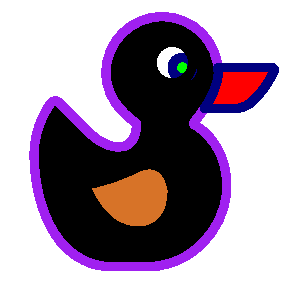
\includegraphics[height=1.4\CharHeight]{shared/qed_duck.pdf}}%
      }%
   }{%
      \providecommand{\myqedsymbol}{$\blacksquare$}%
   }%
}

%-----------------------------------------------------------------------------
% BibLaTeX Setup (Pure Biber, No BibTeX)
%-----------------------------------------------------------------------------
\usepackage[bibencoding=utf8,style=alphabetic,refsegment=chapter,
indexing=cite,
backend=biber]{biblatex}

\ExecuteBibliographyOptions{%
   maxnames = 40,%
   maxalphanames = 4,%
   maxcitenames = 3,%
   minalphanames = 3,%
   minnames = 1,%
   giveninits = true,%
   doi = false,%
   url = false,%
   isbn = false%
}

\renewbibmacro{in:}{}

\AtEveryBibitem{%
   \ifentrytype{inproceedings}{%
      \clearname{editor}%
      \clearlist{editor}%
      \clearfield{editor}%
      \clearlist{publisher}%
      \clearfield{series}%
      \clearlist{location}%
      \clearfield{publisher}%
   }{}%
   \ifentrytype{book}{%
      \clearname{publisher}%
   }{}%
}
\AtEveryCitekey{%
   \ifentrytype{inproceedings}{%
      \clearlist{publisher}%
   }{}%
   \clearname{editor}%
   \clearlist{location}%
}
\DeclareFieldFormat[inproceedings]{date}{}
\DeclareFieldFormat[inproceedings]{pages}{#1, \printfield{year}}
\DeclareFieldFormat[inproceedings]{booktitle}{\mkbibemph{#1,\nopunct}}

\DeclareFieldFormat{journaltitle}{\mkbibemph{#1}\isdot}

\DeclareFieldFormat[article]{number}{\mkbibparens{#1}}
\DeclareFieldFormat[article]{date}{}
\DeclareFieldFormat[article]{pages}{#1, \printfield{year}}
\DeclareFieldFormat[article]{issue}{\nopunct#1}
\renewbibmacro*{issue+date}{%
   \iffieldundef{issue}{}%
   {%
      \printtext{\unspace}%
      (\printfield{issue})%
   }%
   \iffieldundef{pages}%
   {\addcomma\printfield{year}}%
   {}%
}

\renewcommand{\bibpagespunct}{%
   \ifentrytype{article}{\addcolon}{\addcomma}\space%
}

\DeclareFieldFormat[article]{titlecase}{\MakeSentenceCase{#1}}
\DeclareFieldFormat[inproceedings]{titlecase}{\MakeSentenceCase{#1}}
\DeclareFieldFormat[incollection]{titlecase}{\MakeSentenceCase{#1}}
\DeclareFieldFormat[book]{titlecase}{\MakeSentenceCase{#1}}

\renewbibmacro*{journal}{%
   \iffieldundef{journaltitle} {} {\printtext[journaltitle]{%
         \printfield[myplain]{journaltitle}%
         \setunit{\subtitlepunct}%
         \printfield[myplain]{journalsubtitle}}}}
\DeclareFieldFormat{myplain}{#1}

\renewbibmacro*{booktitle}{%
   \ifboolexpr{ test {\iffieldundef{booktitle}} and test
      {\iffieldundef{booksubtitle}} } {} {\printtext[booktitle]{%
         \printfield[myplain]{booktitle}%
         \setunit{\subtitlepunct}%
         \printfield[myplain]{booksubtitle}}%
      \newunit}%
   \printfield{booktitleaddon}}

\renewbibmacro*{volume+number+eid}{%
   \setunit*{\addcomma\addspace}%
   \printfield{volume}%
   \printfield{number}%
   \setunit{\addcomma\space}%
   \printfield{eid}%
}

\newbibmacro{string+doi}[1]{%
   \iffieldundef{doi}{%
      \iffieldundef{url}{%
         #1%
      }{%
         \href{\thefield{url}}{#1}%
      }%
   }{%
      \href{http://dx.doi.org/\thefield{doi}}{#1}}%
}
\DeclareFieldFormat*{title}{\usebibmacro{string+doi}{\mkbibemph{#1}}}
\renewcommand*{\multicitedelim}{\addcomma\space}
\DeclareFieldFormat[inproceedings]{title}{\usebibmacro{string+doi}{{#1}}}
\DeclareFieldFormat[article]{title}{\usebibmacro{string+doi}{{#1}}}
\DeclareFieldFormat[incollection]{title}{\usebibmacro{string+doi}{{#1}}}
\DeclareFieldFormat[book]{titlecase}{{#1}}

\DeclareCiteCommand{\tcite}%
{\usebibmacro{prenote}}%
{\usebibmacro{citeindex}\usebibmacro{cite}}%
{\multicitedelim}%
{\usebibmacro{postnote}}

%-----------------------------------------------------------------------------
% Hyperref & Visual Formatting
%-----------------------------------------------------------------------------
\usepackage{hyperref}
\hypersetup{%
   breaklinks,%
   colorlinks=true,%
   linkcolor=[rgb]{0.45,0.0,0.0},%
   citecolor=[rgb]{0,0,0.45}%
}

\definecolor{DeepNavy}{HTML}{002366}
\definecolor{RoyalBlue}{HTML}{004E92}
\definecolor{SteelBlue}{HTML}{4682B4}
\definecolor{TealBlue}{HTML}{008080}
\definecolor{DarkSlate}{HTML}{2F4F4F}
\definecolor{DustyGrey}{HTML}{696969}

\makeatletter
\AtBeginDocument{\let\@elt\relax}
\makeatother

\headstyles{bringhurst}
\chapterstyle{dash}

\renewcommand{\chapnamefont}{\normalfont\huge\bfseries\color{DeepNavy}}
\renewcommand{\chapnumfont}{\normalfont\huge\bfseries\color{DeepNavy}}
\renewcommand{\chaptitlefont}{\normalfont\Huge\bfseries\color{DeepNavy}}

\counterwithin{footnote}{chapter}

\setsubparaheadstyle{\normalfont\normalsize\itshape\color{DustyGrey}}
\setlength{\beforechapskip}{-20pt} 
\setlength{\afterchapskip}{30pt}
\setsecnumformat{\csname the#1\endcsname.\quad}

%-----------------------------------------------------------------------------
% Standalone Chapter vs Master Book Modes
%-----------------------------------------------------------------------------
\newcommand{\Copyright}{This work is licensed under the Creative Commons Attribution-Noncommercial 3.0 License. To view a copy of this license, visit \url{http://creativecommons.org/licenses/by-nc/3.0/} or send a letter to Creative Commons, 171 Second Street, Suite 300, San Francisco, California, 94105, USA.}

\newcommand{\RealChapterEndInner}{%
   {%
      \begingroup%
      \emergencystretch=1em%
      \printbibliography[heading=subbibliography,segment=\therefsegment]{}%
      \endgroup%
   }%
}

\providecommand{\BookMode}[1]{}
\providecommand{\StandAloneMode}[1]{#1}

\ifx\bookMode\undefined
   % STANDALONE CHAPTER MODE
   \renewcommand{\StandAloneMode}[1]{#1}
   \renewcommand{\BookMode}[1]{}

   \newcommand{\ChapterNumPage}[2]{%
      \if\relax\detokenize{#1}\relax
         \setcounter{chapter}{0}%
      \else\ifnum#1>0
         \setcounter{chapter}{\numexpr#1-1\relax}%
      \else
         \setcounter{chapter}{0}%
      \fi\fi
      \if\relax\detokenize{#2}\relax
         \setcounter{page}{1}%
      \else\ifnum#2>0
         \setcounter{page}{#2}%
      \else
         \setcounter{page}{1}%
      \fi\fi
   }

   \DeclareRobustCommand{\setheadingcolor}{\color{RoyalBlue}}
   \setsecheadstyle{\setheadingcolor\normalfont\Large\bfseries}
   \setsubsecheadstyle{\normalfont\large\bfseries\color{SteelBlue}}
   \setsubsubsecheadstyle{\normalfont\normalsize\bfseries\color{TealBlue}}
   \setparaheadstyle{\normalfont\normalsize\bfseries\color{DarkSlate}}

   \DeclareDocumentCommand{\Chapter}{s o m}{%
      \IfBooleanTF{#1}{%
         \IfValueTF{#2}{\chapter*[]{#2}}{\chapter*[]{#3}}%
      }{%
         \IfValueTF{#2}{\chapter*[]{#2}}{\chapter[]{#3}}%
      }%
      \setcounter{footnote}{0}%
   }
   \newcommand{\ChapterPrefix}{}
   \newcommand{\ChapterGen}{\pagestyle{plain}\vspace*{-0.7cm}}
   \newcommand{\ChapterEnd}{%
      \RealChapterEndInner{}%
      \end{document}%
   }

   \renewcommand{\File}[1]{#1}
   \renewcommand{\RootFile}[1]{../#1}
\else
   % MASTER BOOK MODE
   \renewcommand{\StandAloneMode}[1]{}
   \renewcommand{\BookMode}[1]{#1}

   \newcommand{\ChapterNumPage}[2]{}

   \DeclareDocumentCommand{\Chapter}{s o m}{%
      \IfBooleanTF{#1}{%
         \IfValueTF{#2}{\chapter*[#2]{#3}}{\chapter*{#3}}%
         \ifx\Dir\undefined\else
            \typeout{CHAPTER_MAP: \Dir/\CurrentChapFile => chap: 0, page: \thepage}%
         \fi
      }{%
         \IfValueTF{#2}{\chapter[#2]{#3}}{\chapter{#3}}%
         \ifx\Dir\undefined\else
            \typeout{CHAPTER_MAP: \Dir/\CurrentChapFile => chap: \thechapter, page: \thepage}%
         \fi
      }%
   }
   \newcommand{\ChapterPrefix}{%
      \vspace{-1cm}%
      \subsection*{\small
         {598 - Class notes for Randomized Algorithms}\\
         {Sariel Har-Peled}\\
         {\today}}%
   }
   \newcommand{\ChapterGen}{}
   \newcommand{\ChapterEnd}{\RealChapterEndInner{}}

   \renewcommand{\File}[1]{\Dir/#1}
   \renewcommand{\RootFile}[1]{#1}

   \newcommand{\InputChap}[2]{%
      \def\Dir{#1}%
      \def\CurrentChapFile{#2}%
      \typeout{}%
      \typeout{------------------------------------------------------------}%
      \typeout{PROCESSING FILE: #1/#2}%
      \typeout{}%
      \input{#1/#2}%
   }
\fi

%-----------------------------------------------------------------------------
% Fragments & Quotes
%-----------------------------------------------------------------------------
\newcommand{\InputExt}[1]{%
   \IfFileExists{#1}%
   {\input{#1}}%
   {\IfFileExists{../#1}%
      {\input{../#1}}%
      {\IfFileExists{../../#1}%
         {\input{../../#1}}%
         {\typeout{ERROR: Unable to find #1}}%
      }%
   }%
}
\newcommand{\FragmentName}[1]{\RootFile{fragment/#1.tex}}

\newwrite\FragOutHandle
\newwrite\FragProbeOut
\newread\FragProbeIn
\newif\ifInJunkDir
\InJunkDirfalse

% Detect whether XeTeX was invoked with -output-directory=junk
\edef\FragProbeSecret{\number\uniformdeviate 1000000}
\immediate\openout\FragProbeOut=frag_probe.tmp
\immediate\write\FragProbeOut{\FragProbeSecret}
\immediate\closeout\FragProbeOut

\openin\FragProbeIn=junk/frag_probe.tmp
\ifeof\FragProbeIn
  \InJunkDirfalse
\else
  \read\FragProbeIn to \FragReadSecret
  \closein\FragProbeIn
  \def\trimspace#1 {#1}
  \edef\FragReadSecretClean{\expandafter\trimspace\FragReadSecret}
  \ifx\FragReadSecretClean\FragProbeSecret
    \InJunkDirtrue
  \else
    \InJunkDirfalse
  \fi
\fi

\newcommand{\FragWritePrefix}{%
  \ifx\bookMode\undefined
    % Standalone chapter mode
    \ifInJunkDir ../../fragment/\else ../fragment/\fi
  \else
    % Master book mode
    \ifInJunkDir ../fragment/\else fragment/\fi
  \fi
}

\DeclareDocumentEnvironment{fragment}{m +b}{%
   \immediate\openout\FragOutHandle=\FragWritePrefix#1.tex
   \immediate\write\FragOutHandle{\unexpanded{#2}}%
   \immediate\closeout\FragOutHandle
   #2%
}{}

\makeatletter
\DeclareDocumentCommand{\IncFragment}{m}{%
   \begingroup
      \let\label\@gobble
      \InputExt{\FragmentName{#1}}%
   \endgroup
}
\makeatother

\newcommand{\QuoteOpen}{}
\newcommand{\QuoteClose}{}
\newcommand{\QuoteWrite}[2]{}

\newcommand{\Quote}[2]{%
   \SaveIndent
   \QuoteWrite{#1}{#2}%
   \begin{center}%
      {\footnotesize
         \begin{quote}
             \RestoreIndent
             {#1}\\
             \hspace*{2cm}-- {#2.}
         \end{quote}%
      }%
      \index{quotation!#2}%
   \end{center}%
   \bigskip
}

\newcommand{\QuotePExt}[3]{%
   \hfill%
   \begin{minipage}{0.95\linewidth}%
       \footnotesize {#1}%
       \rule{\linewidth}{0.3mm}%
       \hfill #2, #3%
   \end{minipage}%
}

\epigraphfontsize{\small\itshape}
\setlength{\epigraphwidth}{0.6\textwidth}
\newcommand{\QuoteExt}[3]{%
   \vspace*{-1.6cm}%
   \epigraph{{\footnotesize #1}}{{#2}, {#3}}%
   \vspace*{-1.2cm}%
}

\providecommand{\delX}[1]{{\color{red}\sout{#1}}}
\providecommand{\newX}[1]{{\color{blue}#1}}
\providecommand{\chgY}[2]{{\color{red}\sout{#1}}{\color{blue}#2}}
\providecommand{\remX}[1]{{\color{purple}\textbf{[Remark: #1]}}}
\newcommand{\SpellIgnore}[1]{#1}
\newcommand{\EQ}{\mathrel{\;\;=\;\;}}

%-----------------------------------------------------------------------------
% Save a symbol that we know is going to get redefined.
\def\savesymbol#1{%
  \expandafter\let\expandafter\origsym\expandafter=\csname#1\endcsname
  \expandafter\let\csname orig#1\endcsname=\origsym
  \expandafter\let\csname#1\endcsname=\relax
}

% Restore a previously saved symbol, and rename the current one.
\def\restoresymbol#1#2{%
  \expandafter\let\expandafter\newsym\expandafter=\csname#2\endcsname
  \expandafter\global\expandafter\let\csname#1#2\endcsname=\newsym
  \expandafter\let\expandafter\origsym\expandafter=\csname orig#2\endcsname
  \expandafter\global\expandafter\let\csname#2\endcsname=\origsym
}

\usepackage{pictex}%
\savesymbol{triangle}%
\usepackage{tree}%
\restoresymbol{TreePKG}{triangle}%

% Definitions absorbed from sbook.sty
\providecommand{\MdPrc}{\nu}

\providecommand{\TwoFiguresBase}[4]{%
   \begin{tabular}{cc}
      \begin{minipage}{0.48\linewidth}
          \begin{center}
              {{{#1}}}
          \end{center}
      \end{minipage}
      &
      \begin{minipage}{0.48\linewidth}
          \begin{center}
              {{#3}}
          \end{center}
      \end{minipage}
      \\
      {#2} & {#4}
   \end{tabular}%
}

\providecommand{\TwoFigures}[6]{%
   \begin{tabular}{cc}
      \begin{minipage}{0.48\linewidth}
          \begin{center}
              {\IncludeGraphics[#1]{{#2}}}
          \end{center}
      \end{minipage}
      &
      \begin{minipage}{0.48\linewidth}
          \centerline{\IncludeGraphics[#4]{{#5}}}
      \end{minipage}
      \\
      {#3} & {#6}
   \end{tabular}%
}

\providecommand{\ThreeFigures}[6]{%
   \begin{tabular}{ccc}
        \begin{minipage}{0.30\linewidth}
            \IncludeGraphics[width=5.1cm]{{#1}}\\
        \end{minipage}
        &
        \begin{minipage}{0.30\linewidth}
            \IncludeGraphics[width=5.1cm]{{#2}}\\
        \end{minipage}
        &
        \begin{minipage}{0.30\linewidth}
            \IncludeGraphics[width=5.1cm]{{#3}}\\
        \end{minipage}
        \vspace{-1cm}
        \\
        {#4} & {#5}& {#6}
   \end{tabular}%
}

%-----------------------------------------------------------------------------
\providecommand{\remove}[1]{}
\providecommand{\NotAMSMode}[1]{#1}
\providecommand{\Solution}[1]{}
\providecommand{\Version}[1]{\hfill{Version: #1}}
\providecommand{\Distor}{\mathrm{dist}}
\providecommand{\Hardness}[1]{(h:#1)}
\providecommand{\QuoteOptExt}[3]{\QuoteExt{#1}{#2}{#3}}
\providecommand{\Hypercube}{\EuScript{H}}
\providecommand{\emphiC}[1]{\emphic{#1}{#1}}
\providecommand{\CoverTime}{\EuScript{C}}
\providecommand{\Nbr}{\Gamma}
\providecommand{\CommuteTime}[2]{\mathbf{CT}_{#1#2}}
\providecommand{\Resistance}{\mathbf{R}}
\providecommand{\EffectResist}[2]{\mathbf{R}_{#1#2}}
\providecommand{\NetworkE}{\EuScript{N}}
\providecommand{\trinom}[4]{\binom{#1}{#2 \;\; #3 \;\; #4}}
\providecommand{\Ranges}{\EuScript{R}}
\providecommand{\CClass}[1]{\ensuremath{\mathbf{#1}}}
\providecommand{\coCClass}[1]{\ensuremath{\mathrm{co-}}\CClass{#1}}
\providecommand{\CX}{\EuScript{C}}
\providecommand{\packet}{\mathbf{c}}
\providecommand{\packetA}{\mathbf{d}}
\providecommand{\mopt}{m_{\mathrm{opt}}}
\providecommand{\girth}{\mathop{\mathrm{girth}}}
\providecommand{\CR}{\mathop{\mathrm{cr}}}
\providecommand{\TRUE}{{\textcolor[named]{RedViolet}{\textsf{TRUE}}}\xspace}
\providecommand{\FALSE}{{\textcolor[named]{RedViolet}{\textsf{FALSE}}}\xspace}
\providecommand{\Part}[1]{\part{#1}}
\providecommand{\Section}[1]{\section{#1}}
\providecommand{\SubSection}[1]{\subsection{#1}}
\providecommand{\SubSubSection}[1]{\subsubsection{#1}}
\providecommand{\Exercise}[5]{%
\begin{exercise_h}[#1]%
   \exelab{#3}{}%
   #4%
\end{exercise_h}%
}
\providecommand{\si}[1]{#1}
\providecommand{\myParagraph}[1]{\noindent\textbf{#1}}
\providecommand{\DefName}[1]{#1}
\providecommand{\deflabel}[1]{def_#1}
\providecommand{\Description}[1]{}

%-----------------------------------------------------------------------------
% Mathematical Notations & Environments (from notations.sty)
%-----------------------------------------------------------------------------
%-----------------------------------------------------------------------------
% List environments (questions & compactenum)
%-----------------------------------------------------------------------------

\newlist{compactenumA}{enumerate}{5}%
\setlist[compactenumA]{topsep=0pt,itemsep=-1ex,partopsep=1ex,parsep=1ex,%
   label=(\Alph*)}%

\newlist{compactenumI}{enumerate}{5}%
\setlist[compactenumI]{topsep=0pt,itemsep=-1ex,partopsep=1ex,parsep=1ex,%
   label=(\Roman*)}%

\newlist{compactenuma}{enumerate}{5}%
\setlist[compactenuma]{topsep=0pt,itemsep=-1ex,partopsep=1ex,parsep=1ex,%
   label=(\alph*)}%

\newlist{compactitem}{enumerate}{5}%
\setlist[compactitem]{topsep=0pt,itemsep=-1ex,partopsep=1ex,parsep=1ex,%
   label=\textbullet}%

\newlist{compactenumi}{enumerate}{5}%
\setlist[compactenumi]{topsep=0pt,itemsep=-1ex,partopsep=1ex,parsep=1ex,%
   label=(\roman*)}%

\setcounter{secnumdepth}{5}

\newcommand{\HST}{\TermI{HST}\xspace}
\newcommand{\Term}[1]{\textsf{#1}}
\newcommand{\TermI}[1]{\Term{#1}\index{#1@\Term{#1}}}

\DeclareMathAlphabet{\mathpzc}{OT1}{pzc}{m}{it}

\newcommand{\seg}{\mathsf{s}}

\newcommand{\Diam}{\mathrm{diam}}
\newcommand{\diam}{\mathrm{diam}}

\newcommand{\Copt}{C_{\mathrm{opt}}}
\newcommand{\CenterPnt}{\mathrm{cen}}

\newcommand{\parent}{\overline{\mathrm{p}}}
\newcommand{\parentX}[2][\!]{\parent\pth[#1]{#2}}

\newcommand{\FMS}{\Mh{\EuScript{X}}\index{metric space}}  
\newcommand{\FMSB}{\Mh{\EuScript{Y}}\index{metric space}}  
\newcommand{\FastCut}{\Algorithm{FastCut}\xspace}
\newcommand{\MinCut}{\Algorithm{MinCut}\xspace}
\newcommand{\MinCutRep}{\Algorithm{MinCutRep}\xspace}
\newcommand{\Contract}{\Algorithm{Contract}\xspace}

\newcommand{\Grid}{\mathrm{G}}
\newcommand{\ClosestPair}{\mathcal{CP}}
\newcommand{\SphereChar}{\ensuremath{\mathbb{S}}}
\newcommand{\Sphere}[1]{{\SphereChar^{(#1)}}}

\newcommand{\PntSet}{{\Mh{\mathsf{P}}}}%
\providecommand{\PntSetA}{{\Mh{\mathsf{Q}}}}%

\newcommand{\query}{\mathcalb{q}}

\newcommand{\pnt}{\mathsf{p}}
\newcommand{\pntA}{\mathsf{u}}
\newcommand{\pntB}{\mathsf{v}}
\newcommand{\pntC}{{\mathsf{x}}}
\newcommand{\pntD}{{\mathsf{y}}}
\newcommand{\pntE}{{\mathsf{z}}}

\newcommand{\pntCoord}{\Mh{p}}
\newcommand{\pntCoordA}{\Mh{q}}

%%%%%%%%%%%%%%%%%%%%%%%%%%%%%%%%%%%%%%%%%%%%%%%%%%%%%%%%%%%%%%%%%%%%% 
%%%%%%%%%%%%%%%%%%%%%%%%%%%%%%%%%%%%%%%%%%%%%%%%%%%%%%%%%%%%%%%%%%%%%
% Markov chain notations.

\newcommand{\MCSpc}{\Mh{\mathtt{S}}}
\newcommand{\MCPrb}{\Mh{\mathtt{P}}}
\newcommand{\MCPrbY}[2]{\MCPrb_{#1#2}}
\newcommand{\MCPrbM}{\Mh{\mathbf{P}}}%
\newcommand{\MCPrbT}[3]{\MCPrb_{#1#2}^{(#3)}}
\newcommand{\MCFPrbT}[3]{\Mh{\mathtt{r}}_{#1#2}^{(#3)}}
\newcommand{\MCVstProb}[2]{\Mh{\mathtt{f}}_{#1#2}}
\newcommand{\MCExSteps}[2]{\Mh{\mathtt{h}}_{#1#2}}
\newcommand{\MCPVec}[1]{\mathbf{q}^{(#1)}}
%%%%%%%%%%%%%%%%%%%%%%%%%%%%%%%%%%%%%%%%%%%%%%%%%%%%%%%%%%%%%%%%%%%%%

\newcommand{\Spread}{\Phi}
\newcommand{\VC}{\ensuremath{\mathsf{VC}}\xspace}
\newcommand{\MC}{\ensuremath{\mathsf{MC}}\xspace}
\newcommand{\hyperplane}{h}

\newcommand{\QuickSort}{\Algorithm{QuickSort}\xspace}
\newcommand{\Alg}{\Algorithm{Alg}\xspace}

\newcommand{\Graph}{\Mh{\mathsf{G}}}%
\newcommand{\GraphB}{\mathsf{H}}
\newcommand{\GraphC}{\mathsf{K}}
\newcommand{\GraphD}{\mathsf{F}}

\providecommand{\G}{}
\renewcommand{\G}{\Graph}

\newcommand{\RLP}{\ComplexityClass{RLP}\xspace}
\newcommand{\USTCON}{\ComplexityClass{USTCON}}
\newcommand{\STCON}{\overrightarrow{\ComplexityClass{STCON}}}

\newcommand{\Mtrx}{\mathsf{M}}
\newcommand{\TMtrx}{\mathsf{Q}}
\newcommand{\IMtrx}{\mathcal{I}}

\newcommand{\Expander}[3]{$\left[#1,#2,#3\right]$-expander}

\newcommand{\ChartX}[1]{\ensuremath{\chi_{#1}}}
\newcommand{\Field}{\mathbb{F}}
\newcommand{\LSpace}{\mathbb{G}}
\newcommand{\LD}[2]{\mathsf{L{D}}\pth{#1,#2}}
\newcommand{\SEVN}{\widehat{\lambda_2}}
\newcommand{\NX}[2]{#1\!\left[#2\right]}
\newcommand{\Entry}[2]{#1\!\left[#2\right]}
\newcommand{\NXExt}[3]{#1_{#2}\!\left[#3\right]}
\newcommand{\RangeI}[1]{\llbracket #1 \rrbracket}
\newcommand{\DialX}[1]{\gamma\pth{#1}}
\newcommand{\BiDialX}[1]{{\gamma}_2\pth{#1}}

\newcommand{\EV}[1]{\widehat{\lambda_{#1}}}
\newcommand{\TEV}[1]{\widehat{\lambda_{#1}}}
\newcommand{\EVal}{\widehat{\lambda}}
\newcommand{\Basis}{\mathcal{B}}

\newcommand{\ZProd}[2]{\ensuremath{#1 \, \text{\textcircled{z}} #2}}
\newcommand{\RProd}[2]{\ensuremath{#1 \, \text{\textcircled{r}} #2}}

\newcommand{\OneVec}[1]{\mathbf{1}^{#1}}
\newcommand{\DstrbV}[1]{\mathbf{\mathsf{q}}^{(#1)}}
\newcommand{\DstrbE}[2]{\mathsf{q}^{(#1)}_{#2}}

\newcommand{\DEdges}{\widetilde{\Edges}}

\newcommand{\VV}{\Mh{\mathsf{V}}}%
\newcommand{\EE}{\Mh{\mathsf{E}}}%

\newcommand{\Vertices}{\VV}%
\newcommand{\Edges}{\EE}%

\newcommand{\EdgesX}[1]{\Edges\pth{#1}}
\newcommand{\VerticesX}[1]{V\pth{#1}}

\newcommand{\StringX}[1]{\mathsf{s}\pth{#1}}

\newcommand{\BMtrx}{\mathsf{B}}
\newcommand{\WMtrx}{\mathsf{W}}
\newcommand{\NWMtrx}{\overline{\mathsf{W}}}
\newcommand{\Sequence}{\EuScript{S}}

\newcommand{\med}{\mathrm{med}}
\newcommand{\medX}[1]{\Mh{\mathrm{med}}\pth{#1}}

\newcommand{\medianC}{\Mh{\nu}}%

\newlength{\savedparindent}
\newcommand{\SaveIndent}{\setlength{\savedparindent}{\parindent}}
\newcommand{\RestoreIndent}{\setlength{\parindent}{\savedparindent}}

\newcommand{\NNN}{\mathbb{N}}%
\providecommand{\NN}{\mathbb{N}}%
\renewcommand{\Re}{\mathbb{R}}%
\newcommand{\reals}{\Re}%
\newcommand{\ZZ}{\mathbb{Z}}%

\newcommand{\level}{\mathop{\mathrm{level}}}

\providecommand{\TPDF}[2]{\texorpdfstring{#1}{#2}}

\newcommand{\Hint}[1]{\emph{[#1]}}
\newcommand{\Arr}{\mathop{\mathrm{\EuScript{A}}}}

\newcommand{\Array}{\mathcal{T}}%

\newcommand{\dirEdge}[2]{\left({{#1} \rightarrow {#2}} \right)}

%%%%%%%%%%%%%%%%%%%%%%%%%%%%%%%%%%%%%%%%%%%%%%%%%%%%%%%%%%%%%%%%%%%%%%
% Emphasize stuff...
\definecolor{blue25}{rgb}{0, 0, 11}
\newcommand{\emphic}[2]{%
   \textcolor{blue25}{%
      \bfseries{\emph{#1}}}%
   \index{#2}}
\newcommand{\emphi}[1]{\emphic{#1}{#1}}
\newcommand{\emphOnly}[1]{\textcolor{blue25}{\bfseries{\emph{#1}}}}

\definecolor{almostblack}{rgb}{0, 0, 0.3}
\providecommand{\emphw}[1]{{\textcolor{almostblack}{\emph{#1}}}}%

%
%%%%%%%%%%%%%%%%%%%%%%%%%%%%%%%%%%%%%%%%%%%%%%%%%%%%%%%%%%%%%%%%%%%%%%

\newcommand{\volX}[1]{\mathrm{vol}\pth{#1}}

\newcommand{\Interval}{\EuScript{I}}
\newcommand{\IntervalA}{\EuScript{I}}

\newcommand{\Exp}{\mathrm{Exp}}

\let\Ball\undefined
\newcommand{\Ball}{\mathbf{b}}
\newcommand{\hdim}{d}
\newcommand{\Domain}{\mathcal{D}}
\newcommand{\points}[1]{[\bfseries{#1 points}]}
\newcommand{\Event}{\Mh{\EuScript{E}}}%
\newcommand{\EventB}{\Mh{\EuScript{B}}}%
\newcommand{\EventF}{\Mh{\EuScript{F}}}%
\newcommand{\EventG}{\Mh{\EuScript{G}}}%

\newcommand{\distCmd}[1]{\left\| {#1}  \right\|}
\newcommand{\distY}[2]{\distCmd{#1 - #2}}

\newcommand{\NormalC}{\mathbf{N}}
\newcommand{\NormalY}[2]{\NormalC\pth{#1, #2}}%
\newcommand{\NormalDistOneDim}{\NormalC}
\newcommand{\NormalDistX}[1]{\NormalC^{#1}}
\DeclareMathOperator{\lca}{lca}
\newcommand{\RangeSpace}{\Mh{\mathsf{S}}}%
\newcommand{\RangeSpaceA}{\mathsf{T}}

\newcommand{\range}{\mathbf{r}}
\newcommand{\rangeA}{\mathbf{r}'}

\newcommand{\BadProb}{\varphi}

\newcommand{\EntropyChar}{\mathbb{H}}
\newcommand{\Entropy}[1]{\EntropyChar\pth{#1}}
\newcommand{\EntropyX}[1]{\EntropyChar\pth[]{#1}}

\newcommand{\Matrix}{\mathsf{M}}
\newcommand{\MatrixB}{\mathsf{B}}
\newcommand{\MatrixC}{\mathsf{C}}
\newcommand{\MatrixD}{\mathsf{D}}

\renewcommand{\th}{th\xspace}

\newcommand{\Family}{\mathcal{F}}
\newcommand{\FamilyB}{\mathcal{G}}
\newcommand{\FamilyC}{\mathcal{H}}
\newcommand{\FMSC}{\EuScript{Y}\index{metric space}}

\newcommand{\median}{\overline{\mathsf{m}}}
\newcommand{\QuickSelect}{\Algorithm{Quick{}Select}\xspace}

\providecommand{\row}{\mathbf{r}}%
\newcommand{\rowc}{{r}}%

\newcommand{\vecb}{\mathbf{b}}

\newcommand{\vecA}{\mathbf{v}}
\newcommand{\vecB}{\mathbf{u}}
\newcommand{\vecRand}{\mathbf{r}}

\newcommand{\vecH}{\mathbf{h}}
\newcommand{\vecV}{\mathbf{v}}

\newcommand{\vecX}{\mathbf{x}}
\newcommand{\vecY}{\mathbf{y}}

\newcommand{\DistBinom}[2]{\mathrm{Bin}\pth{#1,#2}}

\newcommand{\DistGeom}[1]{\mathrm{Geom}\pth{#1}}

\newcommand{\Sample}{\mathsf{R}}

\newcommand{\lcm}{\mathop{\mathrm{lcm}}}
\newcommand{\bdiv}{\mathop{\mathrm{div}}}%
\newcommand{\divides}{\mid}%
\newcommand{\poly}{\mathrm{poly}}%

\newcommand{\Group}{\mathcal{G}} 
\newcommand{\GroupA}{\mathcal{H}} 

\newcommand{\algGCD}{\Algorithm{EuclidGCD}\xspace}%

\newcommand{\gOp}{\times}%
\newcommand{\gIdent}{\mathsf{i}}%

\newcommand{\ordX}[2][\!]{\mathop{\mathrm{o{r}d}}\pth[#1]{#2}}

\newcommand{\lSym}[2]{%
   \left(
       \ds {#1}\divides{#2}%
   \right) %
}
\newcommand{\jSym}[2]{\left\llbracket%
       \ds {#1}\divides{#2}%
       \right\rrbracket%
}
\newcommand{\Line}{\ell}

\newcommand{\LevelChar}{\mathbb{L}}
\newcommand{\AtMostKLevelChar}{\LevelChar_{\leq k}}
\newcommand{\AtMostKLevel}[1]{\LevelChar_{\leq k} \pth{ #1}}

\newcommand{\LineSet}{\mathsf{L}}%
\newcommand{\ArrX}[1]{\EuScript{A}\pth{#1}}%

\providecommand{\Matousek}{Matou{\v s}ek\xspace}
\providecommand{\Erdos}{Erd{\H o}s\xspace}
\providecommand{\Lovasz}{Lov\'asz\xspace}

\newcommand{\ProblemC}[1]{{\textsf{\textcolor{red}{#1}\index{problem!#1}}}}
\DefineNamedColor{named}{OliveGreen} {cmyk}{0.64,0,0.95,0.40}
\providecommand{\ComplexityClass}[1]{{{\textcolor[named]{OliveGreen}{%
            \textsc{#1}}}}}
\providecommand{\NPHard}{{\ComplexityClass{NP-Hard}}%
   \index{NP!hard}\xspace}
\providecommand{\NPComplete}{\ComplexityClass{NP-Complete}%
   \index{NP!complete}\xspace}
\providecommand{\APXHard}{\ComplexityClass{APX-Hard}%
   \index{APX!Hard}\xspace}
\providecommand{\NPC}{\ComplexityClass{NPC}%
   \index{NP!complete}\xspace}
\providecommand{\NP}{\ComplexityClass{NP}%
   \index{NP}\xspace}
\providecommand{\POLYT}{\ComplexityClass{P}\xspace}

\newcommand{\envFrame}[1]{\begin{center}\fbox{\begin{minipage}[c]{0.75\textwidth}{#1}\end{minipage}}\end{center}}

\newcommand{\mysqrt}[1]{\ts\!\!\sqrt{#1}}
\newcommand{\SegSet}{\mathsf{S}}
\newcommand{\ArrVD}[1]{\Arr^{|} \pth{#1}}
\newcommand{\RIC}{\textsf{RIC}\index{random incremental
      construction}\xspace}
\newcommand{\ArrB}{\EuScript{B}}

\newcommand{\TreeOpt}{\EuScript{T}_\mathrm{opt}}
\newcommand{\TreeOptA}{\EuScript{T}_\mathrm{opt}'}

\newcommand{\DepthExt}[2]{\mathrm{depth}_{#1}\pth{#2}}
\newcommand{\depthX}[1]{\mathrm{depth}\pth{#1}}

\newcommand{\TreeA}{\EuScript{U}}
\newcommand{\TreeB}{\EuScript{V}}

\newcommand{\Trap}{\sigma}
\newcommand{\TrapA}{\sigma'}
\newcommand{\TrapB}{\sigma''}

\newcommand{\SampleA}{\mathsf{R}'}

\newcommand{\AllRegions}{\mathcal{T}}
\newcommand{\RegionsSet}[1]{\mathcal{F}\pth{#1}}
\newcommand{\RegionsHeavy}[2]{\mathcal{F}_{\!\geq#1}\pth{#2}}
\newcommand{\NumOfRegionsZero}[1]{\ExChar \!f\pth{#1}}
\newcommand{\NumOfRegions}[2]{\ExChar\! f_{\!\geq #1}\pth[]{#2}}
\newcommand{\ObjSet}{\mathsf{S}}

\newcommand{\WeightX}[2][\!]{\omega \pth[#1]{#2}}
\newcommand{\Edge}{\mathsf{e}}

\newcommand{\Face}{\mathsf{f}}

\newcommand{\DefSet}[1]{D\pth{#1}}
\newcommand{\KillSet}[1]{K\pth{#1}}

\newcommand{\CSProbFull}[4]{
   \,\rho_{\!\!\stackrel{\rule[-.005cm]{0cm}{0.1cm}}{#1,
       #4}}\pth{\MakeSBig #2,#3}}

\newcommand{\disk}{D}
\newcommand{\diskA}{D'}

\newcommand{\IntervalSet}{\widehat{\mathcal{I}}}

\newcommand{\GroundSet}{\textsf{X}}
\newcommand{\FGroundSet}{\mathsf{x}}
\newcommand{\RangeSet}{{\mathcal{R}}}
\newcommand{\RangeSetA}{\mathcal{R}'}
\newcommand{\MeasureChar}{\overline{m}}
\newcommand{\Measure}[1]{\MeasureChar\pth{#1}}
\newcommand{\sMeasure}[1]{\overline{s}\pth{#1}}

\newcommand{\SetA}{\Mh{S}}%
\newcommand{\SetB}{\Mh{T}}%
\newcommand{\SetC}{\Mh{N}}%

\newcommand{\VCProj}[2]{#1_{|#2}}
\newcommand{\VCDim}{\mathrm{dim}_{\VC}}
\newcommand{\Dim}{\delta}
\newcommand{\DimA}{\delta'}
\newcommand{\PntSetB}{{{\mathsf{Q}}}}
\newcommand{\PntSetC}{{{\mathsf{R}}}}
\newcommand{\Growth}[2]{{\EuScript{G}}_{#1}\pth{#2}}
\newcommand{\ShatterFunc}[1]{\pi_{#1}}
\newcommand{\Distribution}{\EuScript{D}}
\newcommand{\Error}{\EuScript{E}}

\newcommand{\bd}{{\partial}}%
\newcommand{\eps}{{\varepsilon}}%

\newcommand{\clmlab}[1]{\label{claim:#1}}
\newcommand{\clmref}[1]{\HLink{Claim}{claim:#1}}

\newcommand{\CHX}[1]{{\mathcal{CH}}\pth{#1}}

\newcommand{\ts}{\hspace{0.6pt}}

\def\qedsymbol{\myqedsymbol}%

\newcommand{\qedsign}{\hfill{\hfill\myqedsymbol}}
\newcommand{\qedsignBig}{\hfill{\hfill\rule{4mm}{4mm}}}
\newcommand{\QED}{{\hfill{\hfill\qedsymbol}}}

\newcommand{\num}{\alpha}

\newcommand{\NEW}[1]{#1}

\newcommand{\ThreeFiguresExt}[9]{%
   \begin{tabular}{ccc}
     \begin{minipage}{0.31\linewidth}
         \begin{center}
             {\IncludeGraphics[#1]{{#2}}}
         \end{center}
     \end{minipage}
     &
       \begin{minipage}{0.31\linewidth}
           \centerline{\IncludeGraphics[#4]{{#5}}}
       \end{minipage}
     &
       \begin{minipage}{0.31\linewidth}
           \centerline{\IncludeGraphics[#7]{{#8}}}
       \end{minipage}
     \\
     ~\\[-0.2cm]
     {#3} & {#6} & {#9}
   \end{tabular}}

\newcommand{\IncludeGraphics}[2][]{%
   \typeout{}%
   \typeout{Graphics: #2}%
   \typeout{\ includegraphics[#1]{#2}}%
   \includegraphics[#1]{#2}
   \typeout{}%
}

%    -----------------------------------------------------------------
%    -----------------------------------------------------------------
%    -----------------------------------------------------------------
%    Handling references
%    -----------------------------------------------------------------
%    -----------------------------------------------------------------
%    -----------------------------------------------------------------
\newcommand{\HLinkShort}[2]{\hyperref[#2]{#1\ref*{#2}}}
\newcommand{\HLink}[2]{\hyperref[#2]{#1~\ref*{#2}}}
\newcommand{\HLinkPage}[2]{\hyperref[#2]{#1~\ref*{#2}%
      $_\text{p\pageref{#2}}$}}

\newcommand{\HLinkSuffix}[3]{\hyperref[#2]{#1\ref*{#2}{#3}}}
\newcommand{\HLinkPageSuffix}[3]{\hyperref[#2]{#1\ref*{#2}%
      #3$_\text{p\pageref{#2}}$}}

\newcommand{\figlab}[1]{\label{fig:#1}}
\newcommand{\figref}[1]{\HLink{Figure}{fig:#1}}

\newcommand{\exelab}[1]{\label{exer:#1}}
\newcommand{\exeref}[1]{Exercise~\ref{exer:#1}}

\providecommand{\deflab}[1]{\label{def:#1}}
\newcommand{\defref}[1]{\HLink{Definition}{def:#1}}
\newcommand{\defrefY}[2]{\hyperref[def:#2]{#1}}
\newcommand{\defrefpage}[1]{\HLinkPage{Definition}{def:#1}}

\newcommand{\etal}{\textit{et~al.}\xspace}

\newcommand{\obslab}[1]{\label{observation:#1}}
\newcommand{\obsref}[1]{\HLink{Observation}{observation:#1}}
\newcommand{\obsrefY}[2]{\hyperref[observation:#2]{#1}}

\newcommand{\exmlab}[1]{\label{example:#1}}
\newcommand{\exmref}[1]{\HLink{Example}{example:#1}}

\newcommand{\remlab}[1]{\label{rem:#1}}
\newcommand{\remref}[1]{\HLink{Remark}{rem:#1}}%

\newcommand{\chaplab}[1]{\label{chap:#1}}

\newcommand{\itemlab}[1]{\label{item:#1}}
\newcommand{\itemref}[1]{\HLinkSuffix{}{item:#1}{}}

\newcommand{\tedlab}[1]{\label{tedium:#1}}
\newcommand{\tedref}[1]{\HLink{Tedium}{tedium:#1}}%

\newcommand{\factlab}[1]{\label{fact:#1}}%

\newcommand{\alglab}[1]{\label{algorithm:#1}}

\newcommand{\net}{\Mh{\mathcal{N}}}%
      
\newcommand{\lemlab}[1]{\label{lemma:#1}}
\newcommand{\lemref}[1]{\HLink{Lemma}{lemma:#1}}%
\newcommand{\lemrefY}[2]{\hyperref[lemma:#2]{#1}}
\newcommand{\lemrefpage}[1]{\HLinkPage{Lemma}{lemma:#1}}
\newcommand{\lemrefshort}[1]{\HLinkShort{L}{lemma:#1}}

\newcommand{\eqlab}[1]{\label{equation:#1}}
\newcommand{\Eqrefbare}[1]{\HLinkSuffix{(}{equation:#1}{)}}
\newcommand{\Eqref}[1]{\HLinkSuffix{Eq.~(}{equation:#1}{)}}
\newcommand{\Eqrefpage}[1]{\HLinkPageSuffix{Eq.~(}{equation:#1}{)}}

\newcommand{\seclab}[1]{\label{sec:#1}}
\newcommand{\secref}[1]{\HLink{Section}{sec:#1}}
\newcommand{\secrefY}[2]{\hyperref[sec:#2]{#1}}
\newcommand{\secrefpage}[1]{\HLinkPage{Section}{sec:#1}}

\newcommand{\thmlab}[1]{{\label{theo:#1}}}
\newcommand{\thmref}[1]{\HLink{Theorem}{theo:#1}}
\newcommand{\thmrefY}[2]{\hyperref[theo:#2]{#1}}
\newcommand{\thmrefpage}[1]{\HLinkPage{Theorem}{theo:#1}}

\newcommand{\corlab}[1]{\label{cor:#1}}
\newcommand{\corref}[1]{\HLink{Corollary}{cor:#1}}%

%    -----------------------------------------------------------------
%    -----------------------------------------------------------------
%    -----------------------------------------------------------------
%    Handling references
%    -----------------------------------------------------------------
%    -----------------------------------------------------------------
%    -----------------------------------------------------------------

\newcommand{\ceil}[1]{\left\lceil {#1} \right\rceil}
\newcommand{\floor}[1]{\left\lfloor {#1} \right\rfloor}
\newcommand{\brc}[1]{\left\{ {#1} \right\}}
\newcommand{\pth}[2][\!]{\mleft({#2}\mright)}%
\newcommand{\brk}[1]{\mleft[{#1}\mright]}%
\newcommand{\pbrc}[2][\!\!]{#1\left[ {#2} \bigr. \right]}
\newcommand{\pbrcS}[1]{\left[ {#1} \right]}

\newcommand{\dotprod}[2]{{#1}\cdot{#2}}
\newcommand{\DotProd}[2]{\permut{{#1},{#2}}}
\newcommand{\permut}[1]{\left\langle {#1} \right\rangle}

\newcommand{\MakeBig}{}
\newcommand{\MakesBig}{}
\newcommand{\MakeSBig}{}
\newcommand{\MakeVBig}{}

\newcommand{\DistChar}{\Mh{\mathsf{d}}}%
\newcommand{\DistSetY}[2]{\DistChar\pth{#1,#2}}
\newcommand{\distG}[2]{\DistChar_\Graph\pth{#1, #2}}
\newcommand{\DistMtrCharX}[1]{\DistChar_{#1}}

\newcommand{\dY}[2]{\DistChar\pth{#1, #2}}%
\newcommand{\dGY}[2]{\DistChar_\Graph\pth{#1, #2}}%

\newcommand{\cset}{\mathcal{C}}%

\newcommand{\MTR}{\mathcal{M}}
\newcommand{\DistMtr}[2]{\DistChar\pth{#1,#2}}

\newcommand{\dist}[1]{\left\| {#1} \right\|}
\newcommand{\norm}[1]{\left\| {#1} \right\|}

\providecommand{\ds}{\displaystyle}
\newcommand{\sep}[1]{\,\left|\, {#1} \bigr.\right.}%
\newcommand{\sepw}[1]{\left|\, {#1} \right.}%

\newcommand{\ProbExt}[2]{\mathop{\mathbf{Pr}}_{#1}\pbrcx{#2}}
\newcommand{\ProbLTR}{\mathbb{P}}%

\newcommand{\Prob}[1]{\mathop{\ProbLTR} \mleft[ #1 \mright]}%
\newcommand{\ProbCond}[2]{\mathop{\ProbLTR}\!\left[%
       #1 \;\middle\vert\; #2 \right]}
\newcommand{\ProbY}[2]{\ProbLTR^{}_{\!#1}\pbrc{#2}}

\newcommand{\ExChar}{\mathbb{E}}%
\newcommand{\ExSym}{\mathop{\ExChar}}%
\newcommand{\Ex}[2][\!]{\ExSym#1\pbrcx{#2}}
\newcommand{\ExExt}[2]{\ExSym_{#1}\!\pbrcx{#2}}
\newcommand{\ExExtS}[2]{\ExSym_{\substack{#1}}\!\pbrcx{#2}}
\newcommand{\ExCond}[2]{\ExSym\!\left[%
       #1 \;\middle\vert\; #2 \right]}

\newcommand{\VarSymb}{\mathop{\mathbb{V}}}
\newcommand{\Var}[1]{\mathop{\mathbb{V}}\!\pbrcx{#1}}

\newcommand{\pbrcx}[1]{\left[ {#1} \right]}%
\newcommand{\nfrac}[2]{{#1}/{#2}}
\newcommand{\cardin}[1]{\left| {#1} \right|}%

\newcommand\CCancel[2][black]{{\renewcommand\CancelColor{\color{#1}}\cancel{#2}}}

\newcommand{\IncGraphPage}[4][]{%
   \IncludeGraphics[page=#4,#1]{\File{#2/#3}}%
}

\newenvironment{enumEx}{
   \begin{compactenumA}
    }{\end{compactenumA}}

\newcommand{\cl}{{\mathrm{cl}}}

\usepackage[amsmath,thmmarks]{ntheorem}
\theoremseparator{.}%

\newtheorem{theorem:unnumbered}{Theorem}[section]
\newtheorem{theorem}{Theorem}[section]

\newtheorem{observation}[theorem]{Observation}
\newtheorem{conjecture}[theorem]{Conjecture}
\newtheorem{lemma}[theorem]{Lemma}
\newtheorem{corollary}[theorem]{Corollary}
\newtheorem{claim}[theorem]{Claim}
\newtheorem{assumption}[theorem]{Assumption}
\newtheorem{tedium}[theorem]{Tedium}

\theoremstyle{plain}%
\theoremheaderfont{\sffamily}
\theorembodyfont{\upshape}%

\newtheorem{defn}[theorem]{Definition}
\newtheorem{definition}[theorem]{Definition}

\newtheorem*{remark_unnumbered}[theorem:unnumbered]{Remark}%
\newtheorem*{remarks}[theorem]{Remarks}%
\newtheorem{remark}[theorem]{Remark}%
\newtheorem{fact}[theorem]{Fact}%
\newtheorem{example}[theorem]{Example}
\newtheorem{exercise}[theorem]{Exercise}
\newtheorem{problem}[theorem]{Problem}
\newtheorem{algorithm}[theorem]{Algorithm}%
\newtheorem{xca}[theorem]{Exercise}
\newtheorem{openproblem}[theorem]{Open Problem}
\newtheorem{exercise_h}[theorem]{Exercise}

% Proof environments
\theoremheaderfont{\em}%
\theorembodyfont{\upshape}%
\theoremstyle{nonumberplain}
\theoremseparator{}
\theoremsymbol{\myqedsymbol}
\newtheorem{proof}{Proof:}
\newtheorem{proofextin}{Proof}
\newtheorem{altproof}{Alternative proof:}

\theoremsymbol{}
\newtheorem{proofnoqed}{Proof:}

\theoremsymbol{\myqedsymbol}
\theorempreskip{0pt}%
\theorempostskip{0pt}%
\newtheorem{proofof}{Proof of\!}%

\newenvironment{proofExt}[1]{{\emph{#1:}}}{\hfill{\hfill\myqedsymbol}}
\newenvironment{proofnoproof}{{}}{{\hfill{\hfill\myqedsymbol}}}

%%%%%%%%%%%%%%%%%%%%%%%%%%%%%%%%%%%%%%%%%%%%%%%%%%%%%%%%%%%%%%%%%%%%
%%%%%%%%%%%%%%%%%%%%%%%%%%%%%%%%%%%%%%%%%%%%%%%%%%%%%%%%%%%%%%%%%%%%
% Macros to embed figures in text

\newlength{\RecordedWidth}
\newcommand{\RecordWidth}[1]{\settowidth{\RecordedWidth}{#1}}%

\newlength{\msize}%

%-------------------------------------------------------------------
% \minipageWFigure{ TEXT }{ Figure }{ Figure caption/label }
%-------------------------------------------------------------------
\newcommand{\minipageWFigure}[3]{%
   \RecordWidth{#2}%
   \setlength{\msize}{\dimexpr(\textwidth-1.1\RecordedWidth)\relax}
   \noindent%
   \SaveIndent%
   \begin{minipage}{\msize}%
       \RestoreIndent%
       #1
   \end{minipage}%
   \null\hfill%
   \begin{minipage}{\RecordedWidth}
       \null\hfill%
       #2%       

       #3%
   \end{minipage}%
}

\newcommand{\EBRY}[2]{#1_{\langle#2\rangle}}%

\newcommand{\NiceFrac}[2]{%
   {\raisebox{0.2em}{\ensuremath{#1}}\!\!\!}%
   {\rotatebox[origin=c]{-20}{\Big/}}% Rotated /
   {\! \raisebox{-0.2em}{\ensuremath{#2}} }}%

% end - Macros to embed figures in text
%%%%%%%%%%%%%%%%%%%%%%%%%%%%%%%%%%%%%%%%%%%%%%%%%%%%%%%%%%%%%%%%%%%% 
%%%%%%%%%%%%%%%%%%%%%%%%%%%%%%%%%%%%%%%%%%%%%%%%%%%%%%%%%%%%%%%%%%%%

%%%%%%%%%%%%%%%%%%%%%%%%%%%%%%%%%%%%%%%%%%%%%%%%%%%%%%%%%%%%%%%%%%
% Color in math
\providecommand{\Mh}[1]{{#1}}%
\providecommand{\IfColorMath}[2]{#2}%

\IfFileExists{.latex_printer_friendly}{\def\GenPrinterVer{1}}{}%

\ifx\GenPrinterVer\undefined
   \IfFileExists{.latex_color}{\def\GenColorMath{1}}{}
\else
   \renewcommand{\IfPrinterVer}[2]{#1}%
\fi

\ifx\GenColorMath\undefined
\else
\renewcommand{\IfColorMath}[2]{#1}%
\renewcommand{\Mh}[1]{{\textcolor{red}{#1}}}%
\fi
% Color in math - end
%%%%%%%%%%%%%%%%%%%%%%%%%%%%%%%%%%%%%%%%%%%%%%%%%%%%%%%%%%%%%%%%%%

\newcommand{\HSetY}[2]{\Mh{H}\pth{#1, #2}}%
\newcommand{\CHSetY}[2]{\Mh{C}\pth{#1, #2}}%
\newcommand{\Holder}{H\"older\xspace}
\newcommand{\OldOm}{{\mathcal{O}}}
\newcommand{\NewOm}{{\mathcal{N}}}

%%%%%%%%%%%%%%%%%%%%%%%%%%%%%%%%%%%%%%%%%%%%%%%%%%%%%%%%%%%%%%%%%%%%%%%
%---------------------------------------------------------------
\newcommand{\IntRange}[1]{\left\llbracket #1 \right\rrbracket}
\newcommand{\IRX}[1]{\left\llbracket #1 \right\rrbracket}%
\newcommand{\IRY}[2]{\left\llbracket #1:#2 \right\rrbracket}

%---------------------------------------------------------------
%%%%%%%%%%%%%%%%%%%%%%%%%%%%%%%%%%%%%%%%%%%%%%%%%%%%%%%%%%%%%%%%%%%%%%%

\newcommand{\obj}{\Mh{f}}%
\newcommand{\Wg}{\Mh{\omega}}%
\newcommand{\TotalW}{\Mh{W}}%

\newcommand{\rankY}[2]{{#1}_{ \permut{#2}}}%%
\newcommand{\areaX}[1]{\Mh{\mathrm{area}}\pth{#1}}%%

\newcommand{\mybinom}[2]%
{\Bigl(\begin{array}{@{}c@{}}#1\\#2\end{array}\Bigr)}

\providecommand{\Set}[2]{\left\{ #1 \;\middle\vert\; #2 \right\}}
\newcommand*{\biga}[1]{\vcenter{\hbox{\scalebox{1.5}{\ensuremath#1}}}}
\newcommand{\CNF}{\TermI{CNF}\xspace}%
\newcommand{\Tree}{\Mh{T}}%

\DeclareSymbolFont{sfletters}{OML}{cmbrm}{m}{it}

\DeclareMathSymbol{\salpha}{\mathord}{sfletters}{"0B}

%%%%%%%%%%%%%%%%%%%%%%%%%%%%%%%%%%%%%%%%%%%%%%%%%%%%%%%%%%%%%%%%%%%%

\providecommand{\ProblemInd}[2]{\textsf{\textcolor{red}{#1}\index{Problem!#2}}}
\newcommand{\NPProblemInd}[4]{
   \begin{center}
      \vspace{0.6cm}
       \fbox{
          \begin{minipage}{0.9\linewidth}
              \vspace{-0.6cm} \hspace{-0.35cm}
              {\large \bfseries \ProblemInd{#1}{#2}}
              \vspace{+0.2cm}%

              \noindent{\textcolor{blue}{\bfseries \textsf{Instance}}:} {#3}
              
              \noindent{\textcolor{blue}{\bfseries \textsf{Question}:}} {#4}
          \end{minipage}
       }
   \end{center}
   \smallskip
   }

\newcommand{\NPProblemOpt}[4]{\NPProblemInd{#1}{#2}{#3}{#4}}

%%%%%%%%%%%%%%%%%%%%%%%%%%%%%%%%%%%%%%%%%%%%%%%%%%%%%%%%%%%%%%%%%%%%

\newcommand{\Hastad}{H{\aa}stad\xspace}

\newcommand{\ANNbr}{\Term{ANN}\index{approximate nearest neighbor}\xspace}
\newcommand{\LSH}{\TermI{L{S}H}\xspace}

\newcommand{\DS}{\EuScript{D}} % DataStructure
\newcommand{\DSC}{\mathsf{D}} % DataStructure

\newcommand{\distH}[2]{\DistChar_{H}\pth{#1, #2}}
\newcommand{\distHY}[2]{\DistChar_{H}\pth{#1, #2}}

\newcommand{\DSAprxNearNbr}{\ensuremath{\DataStructure{{\approx%
         \text{Near{}}}}}%
   \index{near neighbor!data-structure!approximate}%
}
\newcommand{\DataStructure}[1]{\ensuremath{\DS_{#1}}}
\newcommand{\DistNN}[2]{\DistChar\pth{#1,#2}}
\newcommand{\pntc}{\Mh{{p}}}%

\newcommand{\seq}{{\Mh{M}}}%
\newcommand{\cTimes}{\Mh{\beta}}%

\newcommand{\DSTimes}{\Mh{L}}%
\newcommand{\rad}{\Mh{r}}%

\newcommand{\HypercubeX}[1]{\Hypercube^{#1}}
\newcommand{\kFunctions}[2]{\mathrm{combine}\pth{#1,#2}}
\newcommand{\WEqualChar}{\Bumpeq}
\newcommand{\WEqual}[2]{{#1}\WEqualChar{#2}}
\newcommand{\FamilyAmp}{\FamilyC_{\WEqualChar}}
\newcommand{\PSPACE}{\ComplexityClass{PSPACE}\xspace}%

\newcommand{\PS}{\Mh{P}}%

\newcommand{\PSetFar}{\ensuremath{\PntSet^{}_{\geq}\xspace}}%
\newcommand{\DA}{\Mh{D}}%
\newcommand{\uniqX}[1]{\Mh{\mathrm{uniq}}\pth{#1}}%
\newcommand{\diffX}[1]{\mathop{}\!\mathrm{d}#1}

\newcommand{\Frq}{\Mh{F}}%
\newcommand{\frq}{\Mh{f}}%
\newcommand{\STRM}{\Mh{\mathcal{S}}}%
\newcommand{\strm}{\Mh{{s}}}%

\providecommand{\Turan}{Tur\'an\xspace}
\newcommand{\fGrowX}[1]{\Mh{G}^{}_{\Dim}\pth{#1}}
\newcommand{\CompressFunc}{\mathtt{Compress}}
\newcommand{\RSA}{\Term{RSA}\xspace}
\newcommand{\MST}{\Term{MST}\xspace}
\providecommand{\CClassPP}{\CClass{P{}P}\xspace}
\providecommand{\ID}{\mathrm{id}}

\newcommand{\EncodeFunc}{\text{\ttfamily{Enc}}}
\newcommand{\DecodeFunc}{\text{\ttfamily{Dec}}}
\newcommand{\discX}[1]{\mathrm{disc}\pth{#1}}%

\newcommand{\propertyC}{\psi}%
\newcommand{\propertyX}[1]{\propertyC\pth{#1}}%
\newcommand{\numC}{\Gamma}%

\newcommand{\degreeX}[1]{\mathrm{degree}\pth{#1}}

\newcommand{\ind}{m}

\providecommand{\nequiv}{\not\equiv}
\providecommand{\sqcupplus}{\sqcup^+}

\newcommand{\AlgorithmI}[1]{{\protect\color{RedViolet}{#1}}}

\MakePerPage{footnote} % Resets footnote counter on every page

\allowdisplaybreaks % Allows page breaks inside multiline math environments

%-----------------------------------------------------------------------------
% Bibliography & Document Begin
%-----------------------------------------------------------------------------
\IfFileExists{\jobname.bib}{%
   \addbibresource{\jobname.bib}%
}{%
   \addbibresource{shortcuts.bib}%
   \addbibresource{geometry.bib}%
}
\makeindex
\begin{document}
%
\fi
\ChapterNumPage{16}{136}

\Chapter{Applications of Chernoff's Inequality}
\ChapterPrefix{}
\ChapterGen{}


\section{QuickSort{} is Quick}

We revisit \QuickSort{}. We remind the reader that the running time of
\QuickSort{} is proportional to the number of comparisons performed by
the algorithm. Next, consider an arbitrary element $u$ being
sorted. Consider the $i$\th level recursive subproblem that contains $u$,
and let $S_i$ be the set of elements in this subproblem. We consider $u$
to be \emph{successful} in the $i$\th level, if
$\cardin{S_{i+1}} \leq \tfrac{3}{4}\cardin{S_i}$. Namely, if $u$ is
successful, then the next level in the recursion involving $u$ would
include a considerably smaller subproblem. Let $X_i$ be the indicator
variable which is $1$ if $u$ is successful.

We first observe that if \QuickSort{} is applied to an array with $n$
elements, then $u$ can be successful at most $T = \ceil{\log_{4/3} n}$
times, before the subproblem it participates in is of size one, and the
recursion stops.  As noted, the indicator variables $X_i$ are
independent, and $\Prob{X_i = 1} \geq 1/2$.  Indeed, when a pivot is chosen
uniformly at random from $S_i$, it falls in the middle half of $S_i$ with
probability at least $1/2$. To this end, conceptually divide $S_i$ into
four equal parts (in sorted order of its elements). If the pivot falls in
middle quarters, then both subproblems have size at most
$\tfrac{3}{4}\cardin{S_i}$.  And this probability is regardless of which
subproblem of $S_i$ contains $u$.

If $u$ participates in $v$ levels, we have the random variables
$X_1, \ldots, X_v$. To make things simpler, we extend this
series by adding independent random variables, such that
$\Prob{X_i=1}=1/2$ for $i > v$. Thus, we have an infinite sequence
of independent random $0/1$ variables, each equal to $1$ with
probability at least $1/2$. The question is how many elements in the
sequence we need to read until we get $T$ ones.

\begin{lemma}
    \lemlab{easy:quick:sort}%
    %
    Let $X_1, X_2,\ldots$ be an infinite sequence of independent random
    $0/1$ variables with $\Prob{X_i = 1} \geq 1/2$. Let $M$ be an arbitrary
    parameter. Then the probability that we need to read more than $6M$
    variables of this sequence until we collect $M$ ones is at most
    $2\exp \pth{- M}$.
\end{lemma}

\begin{proof}
    Consider the random variable $Y = \sum_{i=1}^L X_i$, where $L =
    6M$. Its expectation is $3M$, and using the
    \correfY{Chernoff inequality}{Chernoff:0:1}, we
    get
    \begin{align*}
        \alpha%
        &\EQ%
        \Prob{\Bigl. Y \leq M}%
        \leq%
        \Prob{\Bigl.\cardin{Y - 3M} \geq 2M \bigr.}%
        \LEQ%
        2\exp \Bigl(-\frac{2(2M)^2}{ 6M } \Bigr)
        \\&
        \LEQ%
        2\exp\Bigl( -M   \Bigr).
    \end{align*}
\end{proof}


\begin{lemma}
    For any $c \geq 4$, the probability that \QuickSort{} performs more than
    $6c n \ln n$ comparisons is smaller than $2/n^{c-1}$.
\end{lemma}

\begin{proof}
    For \QuickSort{}, we have that if we sort $n$ elements, for
    $M=c \ln n$ with $c \geq 4$ (so that $M \geq T$), the probability that an
    element $u$ will participate in more than $6M$ rounds is at most
    $2\exp( -M) = 2/n^c$, by \lemref{easy:quick:sort}.  There are $n$
    elements being sorted, and as such, by the union bound, the
    probability that any element would participate in more than
    $6 c \ln n$ recursive calls is smaller than $2/n^{c-1}$, by
    \lemref{easy:quick:sort}.  Since each element participates in at most
    one comparison per recursive call it is involved in (as a non-pivot
    compared against the chosen pivot of its subproblem), the total
    number of comparisons performed is at most
    $\sum_{u} 6c \ln n = 6c n \ln n$.
\end{proof}

\section{The minimums they are a-\SpellIgnore{c{h{}an}g{}in}?}

Let $\Pi = \pi_1 \dots \pi_n$ be a random permutation of $\brc{1,
   \dots, n}$. Let $\Event_i$ be the event that $\pi_i$ is the
minimum number seen so far as we read $\Pi$; that is, $\Event_i$ is
the event that $\pi_i = \min_{k=1}^i \pi_k$. Let $X_i$ be the
indicator variable that is one if $\Event_i$ happens. We have already seen,
and it is easy to verify, that $\Ex{X_i} = 1/i$. We are interested in
how many times the minimum might change\footnote{The answer, my
   friend, is blowing in the permutation.}; that is, $Z=\sum_{i=1}^n X_i$,
and how concentrated the distribution of $Z$ is. The following is
perhaps surprising.

\begin{lemma}
    The events $\Event_1, \ldots, \Event_n$ are independent (as such,
    the variables $X_1, \ldots, X_n$ are independent).
\end{lemma}

\begin{proof}
    Exercise.
    % See homework.
\end{proof}
\remove{%
\begin{proof}
    The trick is to think about the sampling process in a different
    way, and then the result readily follows. Indeed, we randomly pick
    a permutation of the given numbers, and set the first number to be
    $\pi_n$. We then, again, pick a random permutation of the
    remaining numbers and set the first number as the penultimate
    number (i.e., $\pi_{n-1}$) in the output permutation. We repeat
    this process until we generate the whole permutation.

    Now, consider $1 \leq i_1 < i_2 < \ldots < i_k \leq n$, and
    observe that
    \begin{math}
        \Prob{\Bigl. \Event_{i_k} \sep{ \Event_{i_1} \cap \ldots \cap
              \Event_{i_{k-1}} }}%
        = \Prob{\Event_{i_k}},%
    \end{math}
    since by our thought experiment, $\Event_{i_k}$ is determined
    before all the other variables $\Event_{i_{k-1}}, \ldots,
    \Event_{i_1}$, and these variables are inherently not affected by
    this event happening or not. As such, we have
    \begin{align*}
        \Prob{\Bigl. \Event_{i_1} \cap \Event_{i_2} \cap \ldots \cap
           \Event_{i_k} }%
        &=%
        \Prob{\Bigl. \Event_{i_k} \sep{ \Event_{i_1} \cap \ldots \cap
              \Event_{i_{k-1}} }} \Prob{ \Event_{i_1} \cap \ldots \cap
           \Event_{i_{k-1}} }%
        \\&%
        =%
        \Prob{\Bigl. \Event_{i_k}} \Prob{\Bigl. \Event_{i_1} \cap
           \Event_{i_2} \cap \ldots \cap \Event_{i_{k-1}} }%
        =%
        \prod_{j=1}^k \Prob{\Event_{i_j}} = \prod_{j=1}^k
        \frac{1}{i_j},
    \end{align*}
    by induction.
\end{proof}
}
%Now, we have that

\begin{theorem}
    Let $\Pi=\pi_1 \ldots \pi_n$ be a random permutation of
    $1, \ldots, n$, and let $Z$ be the number of times that $\pi_i$ is the
    smallest number among $\pi_1, \ldots, \pi_i$, for $i=1,\ldots, n$. Then, for
    $t \geq 2e$, we have that
    \begin{equation*}
        \Prob{Z > 2t + t  \ln n} \leq 1/ n^{t /2}.
    \end{equation*}
\end{theorem}

\begin{proof}
    Follows readily from Chernoff's inequality, as $Z=\sum_i X_i$ is a
    sum of independent indicator variables, and, by linearity of
    expectation, we have
    \begin{align*}
        \mu%
        &\EQ%
        \Ex{\bigl. Z}%
        =%
        \sum_i \Ex{\big. X_i}%
        =%
        \sum_{i=1}^n \frac{1}{i}%
        \leq%
        1 + \int_{x=1}^{n+1} \frac{1}{x} \mathrm{d}x%
        =%
        1 + \ln (n+1)
        \\&\LEQ
        2 + \ln n,
    \end{align*}
    and similarly $\mu \geq \ln n$.  Next, setting $\delta = t-1$, and 
%    \lemref{chernoff:small:delta:1}
    \lemref{chernoff:delta:big}, yields
    \begin{equation*}
        \Prob{ Z > t( \ln n+2)}
        \LEQ 
        \Prob{ \bigl. Z > (1+\delta)\mu } < 2^{-\mu (1 + \delta)}
        <%
        2^{-t \ln n}
        \leq
        n^{-t/2 }.
    \end{equation*}
\end{proof}


\section{Routing in a parallel computer}
\seclab{routing}


Let $\Graph$ be a graph of a network, where every node is a processor.
The processors communicate by sending packets on the edges. Let
$\bigl[0, \ldots, N -1 \bigr]$ denote the vertices (i.e., processors)
of $\Graph$, where $N = 2^n$, and $\Graph$ is the hypercube. As such,
each processor is identified by a binary string
$b_1b_2\ldots b_n \in \brc{0,1}^n$. Two nodes are connected if their
binary strings differ only in a single bit. Namely, $\Graph$ is the
binary \emphOnly{hypercube}\index{hypercube} over $n$ bits.

We want to investigate the best routing strategy for this network
topology. We assume that every processor needs to send a message to a
single other processor. This is represented by a permutation $\pi$,
and we would like to figure out how to send the messages encoded by
the permutation while creating minimum delay/congestion.

Specifically, in our model, every edge has a FIFO queue\footnote{First
   in, first out queue. I sure hope you already knew that.} of the
packets it has to transmit. At every clock tick, the message in front
of the queue gets sent. All the processors start sending their packets
(to the destination specified by the permutation) at the same time.

A routing scheme is \emphOnly{oblivious}\index{oblivious} if every node that has to
forward a packet, inspects the packet, and depending only on the
content of the packet, decides how to forward it. That is, such a
routing scheme is local in nature, and does not take into account
other considerations. Oblivious routing is of course a bad idea---it
ignores congestion in the network, and might insist on routing things
through regions of the hypercube that are ``gridlocked''.


\begin{theorem}[\cite{kkt-tborh-91}]
    For any deterministic oblivious permutation routing algorithm on a
    network of $N$ nodes each of out-degree $n$, there is a
    permutation for which the routing of the permutation takes
    $\Omega\pth{\! \sqrt{N/n}\, }$ units of time (i.e., ticks).
\end{theorem}

\begin{proof}[Sketch]
    The above is implied by an averaging argument: construct, for every
    possible destination, the routing tree of all packets to this specific
    node. Argue that there must be many edges in this tree that are highly
    congested (which is not the permutation routing we are looking for).
    Now, by averaging, there must be a single edge that is congested in
    ``many'' of these trees. Pick a source-destination pair from each one
    of these trees that uses this edge, and complete it into a full
    permutation in the natural way. Clearly, the congestion of the
    resulting permutation is high. For the exact details see~\cite{kkt-tborh-91}.
\end{proof}

\paragraph*{How do we send a packet?}

We use \emphOnly{bit fixing}\index{bit fixing}.  Namely, the packet from node $i$
always goes to the adjacent node that has the first different bit as we
scan the destination string $d(i)$. For example, a packet from
$(0000)$ going to $(1101)$ would pass through $(1000)$, $(1100)$, and
$(1101)$.

\paragraph*{The routing algorithm.}
We assume each edge has a FIFO queue. The routing algorithm is
depicted in \figref{route}.


\begin{figure}
    \begin{center}
        \fbox{\begin{minipage}{0.85\linewidth}
               \Algorithm{RandomRoute}( $v_0,\ldots, v_{N-1}$)\\
               \CodeComment{\qquad// $v_i$: Packet at node $i$
                  to be routed to node $d(i)$.}

              \begin{compactenumi}
                  \item Pick a \emph{random} intermediate destination
                  $\sigma(i)$ from $[0, \ldots, N-1]$. Packet $v_i$
                  travels to $\sigma(i)$.

                  \CodeComment{\qquad// Random sampling done
                     with \emph{\textbf{replacement}}.}


                  \item Wait until all the packets arrive at
                  their intermediate destination.

                  \item Packet $v_i$ travels from $\sigma(i)$
                  to its destination $d(i)$.
              \end{compactenumi}
              % \smallskip
          \end{minipage}}%
       \vspace{-0.61cm}
   \end{center}

   \caption{The routing algorithm}
   \figlab{route}
\end{figure}

\subsection{Analysis}
We analyze only step 1 in the algorithm, as step 3 follows from the
same analysis.  In the following, let $\rho_i$ denote the route taken
by $v_i$ in step 1.

\begin{exercise}
    A packet $v_j$ traveling along a path $\rho_j$ cannot leave a path
    $\rho_i$ and then rejoin it later. Namely, $\rho_i \cap \rho_j$ is a
    (possibly empty) contiguous path.
\end{exercise}

\begin{lemma}
    Let the route of a message $\packet$ follow the sequence of edges
    $\pi = (e_1, e_2, \ldots, e_k)$. Let $S$ be the set of packets
    whose routes pass through at least one of $(e_1, \ldots, e_k)$.
    Then, the delay incurred by $\packet$ is at most $|S|$.
\end{lemma}

\begin{proof}
    A packet in $S$ is said to leave $\pi$ at that time step at which
    it traverses an edge of $\pi$ for the last time. If a packet is
    ready to follow edge $e_j$ at time $t$, we define its \emph{lag}
    at time $t$ to be $t-j$. The lag of $\packet$ is initially zero,
    and the delay incurred by $\packet$ is its lag when it traverses
    $e_k$. We will show that each step at which the lag of $\packet$
    increases by one can be charged to a distinct member of $S$.

    We argue that if the lag of $\packet$ reaches $\ell+1$, some
    packet in $S$ leaves $\pi$ with lag $\ell$. When the lag of
    $\packet$ increases from $\ell$ to $\ell +1$, there must be at
    least one packet (from $S$) that wishes to traverse the same edge
    as $\packet$ at that time step, since otherwise $\packet$ would be
    permitted to traverse this edge and its lag would not increase.
    Thus, $S$ contains at least one packet whose lag reaches the value
    $\ell$.

    Let $\tau$ be the last time step at which any packet in $S$ has
    lag $\ell$. Thus there is a packet $\packetA$ ready to follow edge
    $e_{\mu}$ at $\tau$, such that $\tau - \mu = \ell$. We argue that
    some packet of $S$ leaves $\pi$ at time $\tau$---this establishes
    the lemma since once a packet leaves $\pi$, it would never join it
    again and as such will never again delay $\packet$.

    Since $\packetA$ is ready to follow $e_{\mu}$ at time $\tau$, some packet
    $\omega$ (which may be $\packetA$ itself) in $S$ traverses $e_\mu$ at time
    $\tau$. Now $\omega$ must leave $\pi$ at time $\tau$---if not, some packet will
    follow $e_{\mu+1}$ at time $\tau+1$ with lag $\ell$.  But this
    violates the maximality of $\tau$.  We charge to $\omega$ the increase in the
    lag of $\packet$ from $\ell$ to $\ell+1$. Since $\omega$ leaves
    $\pi$, it will never be charged again. Thus, each member of $S$ whose
    route intersects $\pi$ is charged for at most one delay, establishing
    the lemma.
\end{proof}


% So, let the route of a message $\packet_i$ follow the sequence of
% edges $\rho_i = (e_1, e_2, \ldots, e_k)$.

Let $H_{i j}$ be an indicator variable that is $1$ if $\rho_i$ and
$\rho_j$ share an edge, and $0$ otherwise. The total delay for $v_i$
is at most $\sum_{j \neq i} H_{i j}$.

Crucially, for a fixed $i$, the variables $H_{i1}, \ldots, H_{i N}$ are almost
independent. Formally, they are conditionally independent given the path
$\rho_i$ (i.e., fix $\rho_i$ and then evaluate these variables).  Indeed,
imagine first picking the destination of $v_i$, and let the associated
path be $\rho_i$. Now, pick the destinations of all the other packets in the
network. Since the sampling of destinations is done with replacement,
whether or not the path $\rho_j$ of $v_j$ intersects $\rho_i$, is independent
of whether $\rho_k$ intersects $\rho_i$. Of course, the probabilities
$\Prob{ \smash{H_{ij} = 1}}$ and $\Prob{ H_{ik} = 1}$ are probably
different.  Confusingly, however, $H_{11}, \ldots, H_{N{} N}$ are not
independent. Indeed, imagine $k$ and $j$ being close vertices on the
hypercube. If $H_{ij} =1$, then intuitively it means that $\rho_i$ is
traveling close to vertex $j$ (the source of packet $v_j$), and as such there is a higher
probability that $H_{ik}=1$.


Let
\begin{equation*}
    \rho_i = (e_1, \ldots, e_k),
\end{equation*}
and let $T(e_j)$ be the \emphi{extra load} of $e_j$. That is, $T(e_j)$ is
the number of packets (i.e., paths) that pass through $e_j$ (in addition
to the $i$\th packet). We have that
\begin{equation*}
    \sum_{j \neq i} H_{i j}%
    \leq%
    \sum_{m=1}^{k} T(e_m) \quad \text{ and thus }\quad \Ex{
       \sum_{j \neq i} H_{i j}}%
    \leq%
    \Ex{ \sum_{m=1}^{k} T(e_m)}.
\end{equation*}
Because of symmetry, the variables $T(e)$ have the same distribution
for all the edges of $\Graph$. On the other hand, the expected length
of a path is $n/2$, there are $N$ packets, and there are $N {n}/2$
edges\footnote{Indeed, the hypercube has $N$ vertices, all of degree
   $n$. As such, the number of undirected edges is $N {n}/2$. Note that
   the network has $Nn$ directed edges, but the calculation here considers
   undirected edges.}. We conclude
\begin{equation*}
    \Ex{ T(e)}
    =%
    \frac{\text{Total length of paths}}{\text{\# of edges in graph}}
    =%
    \frac{N (n/2)}{N (n/2)}
    =%
    1.
\end{equation*}

\begin{claim}
    The probability that the delay of the $i$\th packet exceeds $7n$ is
    at most $2^{-7n}$.
\end{claim}
\begin{proof}
    For a fixed path $\rho_i$ of length $k=\cardin{\rho_i}$, let
    $\mu_i = \ExCond{\sum_{j \neq i} H_{ij}}{\rho_i}$. We have
    \begin{align*}
        \mu_i
        &=
        \ExCond{ \smash{\sum\nolimits_{j \neq i}} H_{i j} }{\rho_i}
        \leq
        \ExCond{\Bigl. \smash{\sum\nolimits_{m=1}^{k}} T(e_m) }{\rho_i}
        \\[0.4cm]&%
        =
        {\sum\nolimits_{m=1}^{k}} \ExCond{T(e_m) }{\rho_i } 
        =
        {\sum\nolimits_{m=1}^{k}} 1
        =
        k \leq n.
    \end{align*}
    (In expectation over $\rho_i$, $\Ex{\mu_i} \leq \Ex{k} = n/2$.)
    For a fixed $\rho_i$, by the Chernoff inequality, specifically
    \lemref{chernoff:delta:big}, we have
    \begin{equation*}
        \ProbCond{ \sum_{j \neq i} H_{i j} > 7n }{\rho_i}
        \EQ%
        \ProbCond{ \sum_{j \neq i} H_{i j} >
           \tfrac{7n}{\mu_i} \ts \mu_i }{\rho_i}
        <
        2^{-(7n/\mu_i)\mu_i}
        \leq
        2^{-7n},
    \end{equation*}
    since $1 + \delta = 7n/\mu_i \geq 7 > 2e$, so $\delta > 2e - 1$.
    Taking the expectation over all choices of $\rho_i$ yields the unconditional probability
    $\Prob{\sum_{j \neq i} H_{ij} > 7n} < 2^{-7n}$.
\end{proof}

Since there are $N = 2^n$ packets, we know that with probability at least
$1 - 2^{-6n}$, all packets arrive at their temporary destination with a
delay of at most $7n$.%
Specifically, by the union bound across all $N = 2^n$ packets, the
probability of any packet suffering delay $> 7n$ is at most
$N \cdot 2^{-7n} = 2^n \cdot 2^{-7n} = 2^{-6n}$.

\begin{theorem}
    \thmlab{route}%
    %
    All packets arrive at their (real) destination in $\leq 16n$ time steps,
    with probability at least $1 - 1/N$ (note that this is very
    conservative).
\end{theorem}
\begin{proof}
    In each phase, a packet traverses a path of length at most $n$ with
    delay at most $7n$, taking at most $8n$ time steps. Summing over both
    phases gives at most $16n$ time steps (or $14n$ if delay is bounded
    by $6n$). By the union bound over both phases, the probability that
    all packets arrive within $16n$ steps is at least
    $1 - 2 \cdot 2^{-6n} = 1 - 2^{-(6n-1)} \geq 1 - 1/N$.
\end{proof}

\section{Faraway Strings}

Consider the Hamming distance between binary strings. It is natural to
ask how many strings of length $n$ one can have, such that any pair of
them is of Hamming distance at least $t$ from each other. Consider
two random strings, generated by picking each bit randomly and
independently. Thus, $\Ex{d_H(x,y)} = n/2$, where $d_H(x,y)$ denotes
the Hamming distance between $x$ and $y$. In particular, using the
Chernoff inequality, specifically \corref{Chernoff:0:1}, we have that
\begin{equation*}
    \Prob{\bigl.d_H(x,y) \leq n/2 - \Delta} \leq \exp\pth{ -2\Delta^2 /n}.
\end{equation*}
Next, consider generating $M$ such strings, where the value of $M$
will be determined shortly. Clearly, the probability that some pair of
strings is at distance at most $n/2 - \Delta$, is
\begin{equation*}
    \alpha \leq \binom{M}{2} \exp\pth{ -2\Delta^2 /n} < M^2 \exp\pth{
       -2\Delta^2 /n}.
\end{equation*}
If this probability is smaller than one, then there is some
probability that all the $M$ strings are of distance at least $n/2 -
\Delta$ from each other. Namely, there exists a set of $M$ strings
such that every pair of them is far. We used here the fact that if an
event has probability strictly greater than zero, then there exists
an outcome satisfying it. Thus, set $\Delta = n/4$, and observe that
\begin{equation*}
    \alpha < M^2 \exp\pth{ -2n^2 /16n} = M^2 \exp\pth{ -n /8}.
\end{equation*}
Thus, for $M = \exp(n/16)$, we have that $\alpha < 1$. Indeed,
$M = \lfloor \exp(n/16) \rfloor$, and
$\alpha \leq \binom{M}{2}\exp(-n/8) < \frac{M^2}{2}\exp(-n/8) \leq 1/2 <
1$.  We conclude:
\begin{lemma}
    \lemlab{faraway}%
    %
    There exists a set of $\exp(n/16)$ binary strings of length $n$,
    such that any pair of them is at Hamming distance at least $n/4$
    from each other.
\end{lemma}
\remX{Since $M$ is defined as $\lfloor \exp(n/16) \rfloor$, the set
cardinality is $\lfloor \exp(n/16) \rfloor$, making the integer
quantity explicit.}

This is our first introduction to the beautiful technique known as the
probabilistic method---we will hear more about it later in the
course.


This result also has an interesting interpretation in the Euclidean
setting. Indeed, consider the sphere $\SphereChar$ of radius
$\sqrt{n}/2$ centered at
\begin{equation*}
    (1/2, \dots, 1/2) \in \Re^n.
\end{equation*}
Clearly, all the vertices of the binary hypercube $\brc{0,1}^n$ lie on
this sphere. As such, let $P$ be the set of points on $\SphereChar$ as
generated by \lemref{faraway}. A pair $p,q$ of points of $P$ has
\emph{Euclidean} distance at least
$\sqrt{d_H(p,q)} = \sqrt{n/4} = \sqrt{n}/2$ from each other. We conclude:

\begin{lemma}
    Consider the unit hypersphere in $\Re^n$, formally defined as
    $\SphereChar^{n-1} = \Set{u\in\Re^n}{\norm{u}=1}$. The sphere
    $\SphereChar^{n-1}$ contains a set $Q$ of points, such that each pair
    of points is at (Euclidean) distance at least one from each other,
    and $\cardin{Q} \geq \exp(n/16)$.
\end{lemma}

\begin{proof}
    Translate the point set $P$ by $-(1/2, \dots, 1/2)$ so that the
    sphere is centered at the origin, and then scale it down by a factor
    of $\sqrt{n}/2$.
\end{proof}

\section{Bibliographical notes}


\secref{routing} is based on Section 4.2 in~\cite{mr-ra-95}.  A similar
result to \thmref{route} is known for the case of the wrapped butterfly
topology (which is similar to the hypercube topology but every node has a
constant degree, and there is no clear symmetry). The interested reader
is referred to~\cite{mu-pcrap-05}.  The randomized two-phase routing
scheme via intermediate random destinations is due to
Valiant~\cite{v-sfpc-82}. The high-probability bound for \QuickSort{}
using Chernoff bounds is standard; see Hoare~\cite{h-q-62} for the
original algorithm and Motwani and Raghavan~\cite{mr-ra-95} for the
analysis. The existence of sets of faraway binary strings is closely
related to the Gilbert-Varshamov bound in coding theory~\cite{g-tce-52}.

%%%%%%%%%%%%%%%%%%%%%%%%%%%%%%%%%%%%%%%%%%%%%%%%%%%%%%%%%%%%%%%%%%%%%%%
%%%%%%%%%%%%%%%%%%%%%%%%%%%%%%%%%%%%%%%%%%%%%%%%%%%%%%%%%%%%%%%%%%%%%%%
\section{Exercises}

\Exercise{More binary strings. More!}%
{10}%
{more:binary:strings}%
{%
   \lemref{faraway} is somewhat silly, as one can prove a better bound by
   direct argumentation. Indeed, for a fixed binary string $x$ of length
   $n$, show a bound on the number of strings in the Hamming ball around
   $x$ of radius $n/4$ (i.e., binary strings of distance at most $n/4$
   from $x$). (Hint: interpret the special case of the Chernoff
   inequality as an inequality over binomial coefficients.)

   Next, argue that the greedy algorithm which repeatedly picks a
   string that is at distance $\geq n/4$ from all strings picked so
   far, stops after picking at least $\exp(n/8)$ strings. %
}{}


\StandAloneMode{
   \section{From previous lectures}

   \IncFragment{c_h_r_0_1}%
   \IncFragment{Chernoff_simplified}%
   \IncFragment{chernoff_delta_big}%
   \IncFragment{chernoff_small_delta_1}%
%  \IncFragment{chernoff_delta_big} % Removed duplicate fragment inclusion
}


\ChapterEnd{}

%%% Local Variables:
%%% mode: latex
%%% TeX-master: "chernoff_app_reviewed"
%%% End:
